

\chapter{Résumé}

Les systèmes en matière molle présentent, dans la plupart des cas, des échelles de longueur structurelle allant du nanomètre au micromètre, et sont donc classés dans le domaine de la "nanotechnologie". Les systèmes colloïdaux sont des exemples bien connus pour lesquels cette caractéristique est essentielle pour définir la plage dans laquelle un type de comportement très spécifique se produit. Les colloïdes sont des substances supramoléculaires et submicroniques dispersées dans un milieu qui peut être un liquide ou un gaz. Ils sont beaucoup plus gros que les molécules et, par conséquent, le milieu d'une suspension colloïdale peut souvent être considéré comme un "arrière-plan" en ce qui concerne la gamme de tailles des colloïdes : ce milieu peut être approximé comme un continuum. En même temps, les colloïdes sont suffisamment petits pour présenter une agitation thermique considérable par rapport à l'effet de sédimentation (qui est causé par des forces gravitationnelles qui deviendraient plus importantes pour des particules de taille plus élevée). Les colloïdes ont été découverts pour la première fois par Perrin, qui a détecté le mouvement brownien comme une manifestation visible de l'agitation thermique dans des dispersions de colloïdes de résine dans l'eau \cite{perrin1913atomes}.

Lorsque les particules colloïdales présentent des formes anisotropes, elles peuvent se trouver dans des phases cristallines liquides. Les cristaux liquides sont des substances qui ont l'apparence d'un liquide mais qui possèdent certains niveaux d'arrangement moléculaire semblables à des cristaux. Les cristaux liquides ont été découverts pour la première fois en 1888 par Friedrich Reinitzer, qui a remarqué qu'une substance à base de cholestérol avait deux points de fusion à des températures différentes, chacun d'eux donnant lieu à une phase liquide aux propriétés optiques différentes \cite{reinitzer1888beitrage}. À l'époque de Reinitzer, seules trois phases étaient connues (gaz, liquide et solide). Au fil des ans, on a découvert qu'un grand nombre de substances présentaient de nombreux états de la matière, y compris des phases cristallines liquides qui sont aujourd'hui largement utilisées dans les avancées technologiques telles que les écrans et les thermomètres à cristal liquide \cite{Li_2012}.

La principale différence entre un cristal liquide et les états gazeux, liquide et solide couramment observés est que les propriétés du premier sont anisotropes et varient en fonction de la direction, même si la substance elle-même reste fluide. Ces propriétés uniques sont dues à la forme allongée de ses éléments constitutifs, qui favorisent l'alignement collectif dans une certaine direction. En d'autres termes, les phases cristallines liquides sont des états supplémentaires de la matière, intermédiaires entre le liquide usuel et le solide cristallin, dont l'existence est liée aux degrés de liberté supplémentaires que possèdent les particules anisométriques par rapport aux particules sphériques.


Parmi les nombreuses phases cristallines liquides, on peut trouver différents degrés d'ordre, mis en évidence par exemple par la diffraction des rayons X et de la lumière. Les mesures de ce type permettent de classer ces systèmes en fonction de leur similitude avec la phase liquide ou la phase solide. Considérons, entre autres, les phases cristallines liquides suivantes, représentées dans \fig{frenchfig} :

La phase fluide {\em isotrope} (I) est très similaire aux phases gazeuse et liquide pour les particules sphériques et se caractérise par une absence totale d'ordre positionnel et orientationnel. Au stade immédiatement suivant, nous trouvons la phase {\em nématique} (N), dans laquelle les particules sont réparties de manière homogène sans ordre de position comme dans une phase liquide, mais sont ordonnées dans leur orientation suivant une direction moyenne : le directeur nématique $\bn$. Comme nous le voyons à plusieurs reprises tout au long de cette thèse, les particules, en plus d'être anisotropes, peuvent être chirales. Cela peut être dû à l'arrangement des atomes dans un composé moléculaire, à une forme de particule (hélicoïdale) dans certains systèmes colloïdaux ou à une distribution chirale des charges à la surface des particules, observée par exemple dans  les virus en forme de filament {\em fd} \cite{Gibaud_2017}. Lorsque les particules chirales sont en phase nématique, elles s'organisent en une structure fortement torsadée. Ce cas particulier de phase nématique chirale est souvent appelé {\em cholestérique}.

La phase {\em smectique} (Sm) est plus proche de la phase solide. Dans les cristaux liquides smectiques, les particules sont ordonnées en couches et ne peuvent pas se déplacer librement d'une couche à l'autre. La phase smectique est à son tour divisée en plusieurs types aux propriétés différentes. Par exemple, la phase smectique A (SmA), où les particules peuvent se déplacer librement à l'intérieur des couches comme dans un liquide bidimensionnel, ou la phase smectique B (SmB), où il existe un ordre positionnel à longue distance : à des concentrations plus élevées ou à des températures plus basses, les molécules ont tendance à s'arranger de manière de plus en plus proche d'un réseau cristallin.

Une autre classification des matériaux cristaux liquides est basée sur le mécanisme par lequel ils passent d'un état à l'autre. Les systèmes {\em thermotropes}, principalement formés par des constituants de faible poids moléculaire - et aussi certains polymères -, subissent des transitions de phase dues à des changements de température, puisque les propriétés thermodynamiques de ces espèces dépendent des forces d'attraction entre les molécules. Dans cette thèse, nous nous concentrons principalement sur les cristaux liquides {\em lyotropes}, qui se forment en augmentant la concentration des particules de soluté. C'est le cas des systèmes formés par des nanoparticules synthétiques et biologiques de haut poids moléculaire \cite{sonin1998inorganic,dogic-fraden_fil}, des polymères tels que l'ADN \cite{livolantDNAoverview} ou des surfactants dans un solvant \cite{fontell1981}. Le premier cas est celui étudié dans cette thèse, où le fait que la forme ne soit pas sujette à des fluctuations dues à des changements dans la composition du solvant est une simplification avantageuse par rapport à ses homologues amphiphiles et polymèriques.

Les premiers rapports expérimentaux sur les cristaux liquides lyotropes à base de nanoparticules remontent à la description du comportement cristal liquide du virus de la mosaïque du tabac et de la tomate (TMV) \cite{Bawden,Bernal} et du pentoxyde de vanadium (V$_{2}$O$_{5}$) \cite{Zocher} au début du 20e siècle. Outre ces systèmes de particules en forme de bâtonnets, on a découvert que les particules colloïdales chargées en forme de plaquettes et les particules d'argile présentaient un comportement cristal liquide \cite{Langmuir}. Actuellement, il existe de nombreux autres exemples de cristaux liquides lyotropes dans une grande variété de dispersions de particules colloïdales (principalement en forme de bâtonnets) et de solutions de polymères rigides (voir par exemple \cite{Dierking2020} pour une vue d'ensemble).

\begin{figure}
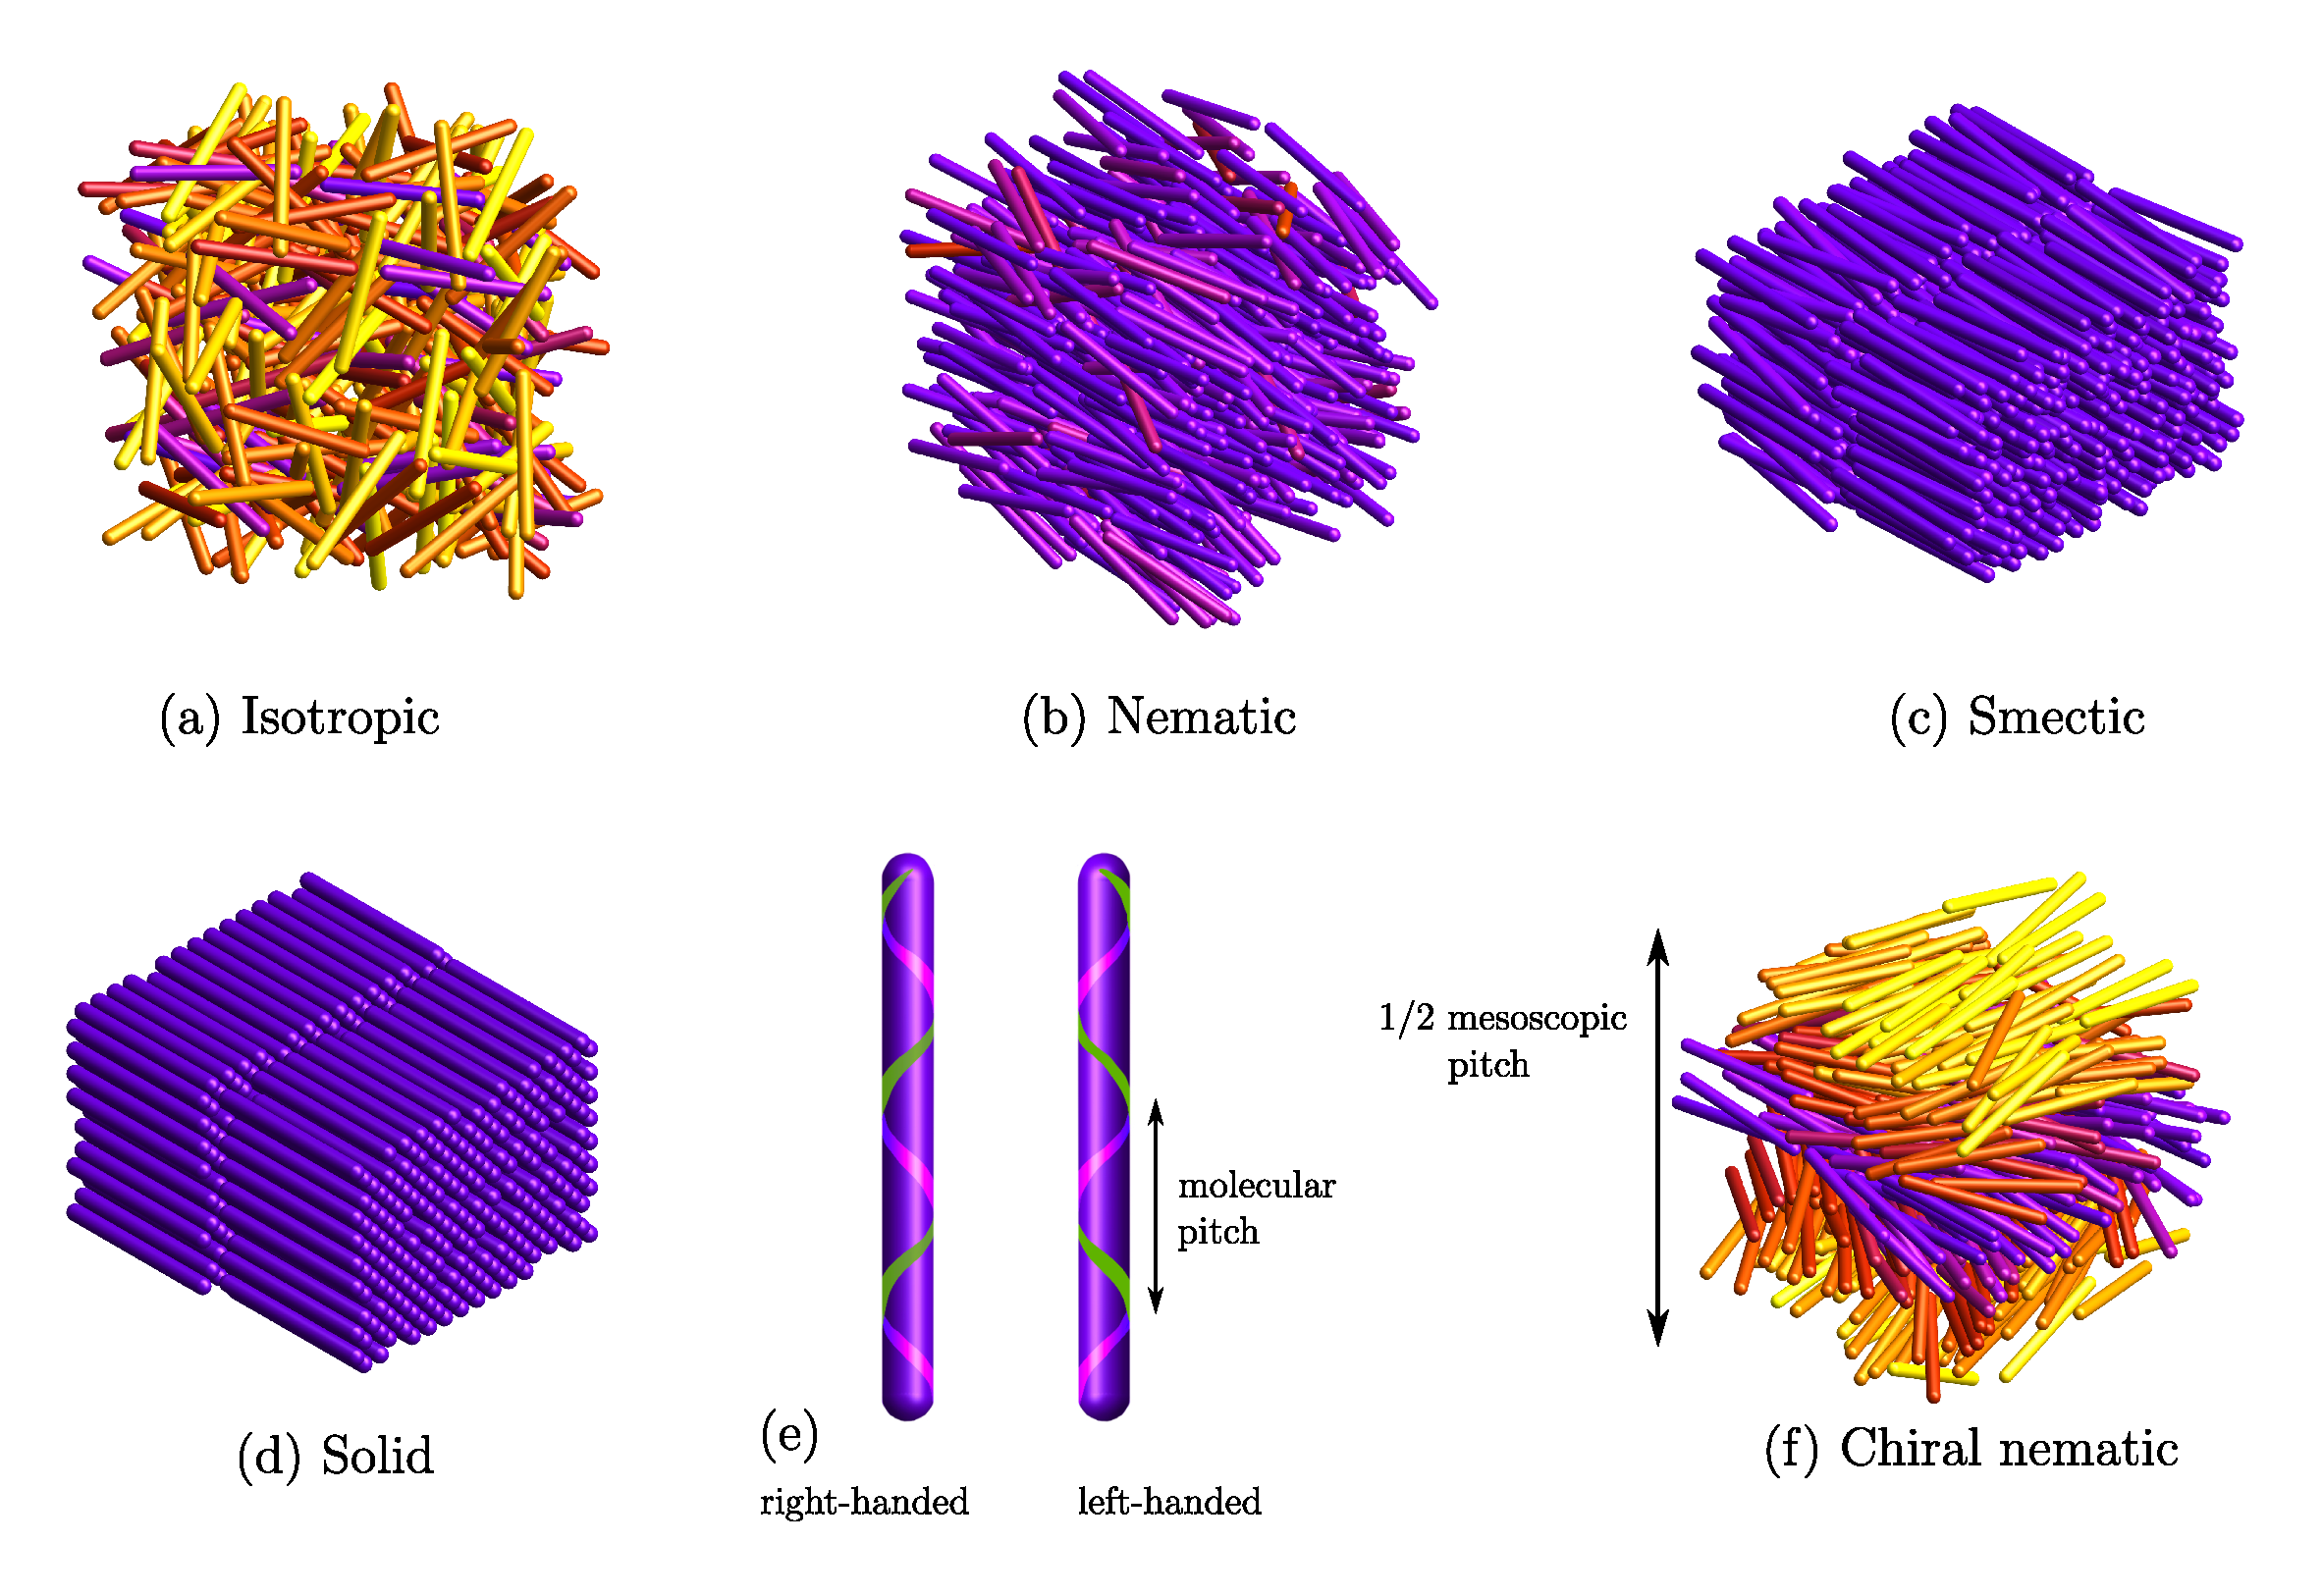
\includegraphics[width= \columnwidth]{figures/chapter-1/phases}
\caption[Exemples de cristaux liquides basiques formés par des molécules ou des nanoparticules en forme de bâtonnets]{ \label{frenchfig} (a)-(d) Exemples de cristaux liquides de base formés par des molécules ou des nanoparticules en forme de bâtonnets. (e) Les cristaux liquides peuvent être formés par des constituant chiraux; (f) ces particules génèrent un type particulier de phase nématique : le nématique chiral. Les implications de la chiralité moléculaire sur la mésostructure hélicoïdale (en particulier, le {\em pitch} mésoscopique) des phases nématiques chirales restent une question difficile.}
\end{figure}

Ce travail de recherche se concentre sur les approches théoriques et numériques pour l'exploration du comportement de phase dans les composés colloïdaux anisotropes, avec un intérêt particulier pour la transition de phase isotrope-nématique de nature {\em entropique}. Cette transition est bien décrite par la théorie d'Onsager, proposée en 1949, qui suppose une similarité entre un gaz et une solution de particules \cite{onsager1949} ; et sera utilisée à plusieurs reprises dans ce manuscrit (plus particulièrement dans les chapitres \ref{disc_polymer} et \ref{hybridLC2}) avec d'autres outils théoriques et numériques pour étudier l'auto-organisation liquide-cristalline de bâtonnets ou de plaquettes colloïdales dans des environnements complexes. Grâce à nos recherches, nous espérons mieux comprendre le comportement de ce type de systèmes et contribuer au domaine plus large de la recherche sur les cristaux liquides.


%L'objectif central de cette thèse est d'étudier théoriquement l'auto-organisation des particules colloïdales de cristaux liquides (LC) avec différentes formes dans divers contextes. Beaucoup des études qui seront décrites dans le reste de cette thèse ont été inspirées par des travaux expérimentaux récents sur des systèmes de colloïdes avec des formes et des interactions bien contrôlées. En particulier, nous mentionnons les travaux expérimentaux de \cite{Grelet2014} sur le comportement de phase et la fonctionnalisation de fluides complexes de bactériophages filamentaires (fd et M13) qui présentent de nombreux phénomènes intéressants laissés ouverts à l'interprétation théorique ; ainsi que les résultats expérimentaux récents \cite{senyuk2021nematoelasticity,mundoor2021} sur la dispersion colloïdale de particules hautement anisotropes immergées dans des hôtes de cristaux liquides moléculaires. Un de nos objectifs principaux dans ce travail est de rendre compte de ces observations expérimentales en construisant des modèles simples mais réalistes pour les systèmes colloïdaux étudiés et en examinant les aspects pertinents de leur comportement de phase.

Le chapitre \ref{introduction} de cette thèse fournit une introduction au contexte et à la portée de la recherche présentée. Il couvre le contexte de mécanique statistique appliquée aux fluides de particules anisométriques {\em dures}. Nous discutons ensuite de l'utilisation des simulations de Monte Carlo de particules dures, en mettant en évidence certaines particularités de telles simulations pour le cas de particules anisométriques. Dans l'ensemble, le chapitre sert de fondement pour le reste de la thèse, en exposant les concepts et les méthodes pertinents pour la recherche présentée dans les chapitres suivants.

Dans le chapitre \ref{disc_polymer}, un modèle théorique est proposé pour explorer le comportement de phase à faible concentration d'un système composé de batônnets peu flexibles liés de manière non covalente et traités comme des {\em living polymers} mélangés à des disques colloïdaux rigides non adsorbants. En utilisant une théorie du second coefficient du viriel qui corrèle les différentes entropies associées aux polymères et aux disques, nous démontrons que de faibles fractions d'additifs discotiques favorisent la formation d'une phase nématique de polymère. À des concentrations plus élevées de disques, cependant, la phase est perturbée par l'alignement collectif des disques en faveur d'un fluide nématique discotique dans lequel les polymères sont dispersés de manière {\em antinématique}. Nous montrons que l'arrangement antinématique des polymères génère une distribution de poids moléculaires non exponentielle et stimule la formation d'espèces oligomériques. À des concentrations suffisantes, les disques facilitent une séparation de phase liquide-liquide qui peut être mise en coexistence simultanée avec les deux phases nématiques fractionnées, fournissant ainsi des preuves d'une coexistence à quatre fluides dans un mélange de particules dures de formes différentes sans forces interparticulaires cohésives. Nous stipulons les conditions dans lesquelles un tel phénomène pourrait être observé expérimentalement.

Les chapitres \ref{hybridLC1} et \ref{hybridLC2} abordent des problèmes liés aux cristaux liquides nématiques moléculaires hybrides. Dans cette partie du travail, nous considérons un système dans lequel les cristaux liquides cholestériques moléculaires sont dopés avec de fines particules colloïdales ayant de grands rapports longueur-largeur. Dans le chapitre \ref{hybridLC1}, nous considérons des insertions individuelles de colloïdes. Nous démontrons que les tiges ont une forte tendance à s'orienter perpendiculairement à l'axe hélicoïdal et au directeur local, conférant ainsi une forte biaxialité locale à la structure cholestérique hybride. Nous argumentons théoriquement que l'anisotropie élastique et l'étalement  de la courbure joue un rôle clé dans la stabilisation de l'ordre orthorhombique local le long de l'hélice. Nos prévisions sont corroborées par des résultats expérimentaux obtenus dans le groupe de I. Smalyukh (Université du Colorado, États-Unis) que nous examinons brièvement. Nous discutons également le cas des disques et trouvons un scénario similaire d'ordre biaxial anormal le long du directeur hélicoïdal pour des disques à ancrage homéotrope immergés dans des hôtes cholestériques à pas court.

Dans le chapitre \ref{hybridLC2}, nous utilisons la théorie d'Onsager pour rendre compte des effets collectifs dans le cas hypothétique où de nombreuses particules colloïdales sont insérées dans le LC hybride. Ce cadre nous permet d'explorer des concentrations de colloïdes qui ne sont plus infiniment petites. Les corrélations entre les colloïdes entraînent des contributions élastiques et entropiques supplémentaires qui interfèrent avec les effets d'ancrage de surface explorés dans le chapitre précédent. Nous considérons deux régimes distincts, à savoir le couplage faible où l'ancrage de surface n'a qu'un impact marginal sur les orientations des colloïdes et le couplage fort où l'énergie de réalignement typique dépasse largement l'énergie thermique. Nous démontrons en couplage faible que les effets collectifs colloïdaux induits par l'interaction stérique colloïde-colloïde peuvent conduire à une séparation de phase liquide-liquide entre deux phases fluides biaxes. Dans le régime de couplage fort, nous soutenons que la force élastique peut faciliter la formation d'états bi-hélicoïdaux où l'organisation hélicoïdale des composants colloïdaux et moléculaires est inégale en pas et même en chiralité.

Finalement, dans le chapitre \ref{twistedrods}, nous utilisons des simulations de Monte Carlo approfondies, complétées par la théorie, pour explorer deux formes de gouttelettes importantes dans la littérature, à savoir la membrane torsadée et le ruban colloïdaux. Dans les expériences, la structure de ruban allongée domine à force chirale élevée. Cependant, dans nos simulations, nous démontrons qu'en augmentant la chiralité, les membranes ont tendance à se transformer en structures à plusieurs domaines composées de plusieurs unités presque circulaires torsadées séparées par des parois $\pi$, tandis que la transition en rubans torsadés est entravée par la forte tension de surface subie par la gouttelette. Nous complétons nos simulations avec des descriptions théoriques microscopiques simples pour les deux morphologies de gouttelettes, ce qui nous permet de prédire l'évolution de l'angle de torsion à travers les membranes. Pour les rubans, notre théorie simple fournit des prévisions génériques pour la largeur de ruban typique, la torsion interne et l'angle d'inclinaison des bords qui sont en accord avec les observations expérimentales de rubans torsadés composés de bâtonnets de virus {\em fd} mélangés avec du dextran.

{\large\textbf{Mots clés:}} cristal liquide; colloïde; théorie d'Onsager; Hard Particle Monte Carlo